% Based on template: http://www.maths.lth.se/matematiklth/exjobb/exjobbarresurs/index.html

\documentclass{IEEEtran}

\usepackage[smartEllipses]{markdown}  % For markdown
\usepackage{hyperref}
\usepackage{comment}
\usepackage{xargs}
\usepackage[colorinlistoftodos, prependcaption, textsize=tiny]{todonotes}

% From: https://tex.stackexchange.com/a/178806/36302
\newcommandx{\add}[2][1=]{\todo[linecolor=red, backgroundcolor=red!25, bordercolor=red, inline, #1]{Add: #2}}
\newcommandx{\unsure}[2][1=]{\todo[linecolor=red, backgroundcolor=red!25, bordercolor=red, #1]{Unsure: #2}}
\newcommandx{\change}[2][1=]{\todo[linecolor=blue, backgroundcolor=blue!25, bordercolor=blue, #1]{Change: #2}}
\newcommandx{\info}[2][1=]{\todo[linecolor=OliveGreen, backgroundcolor=OliveGreen!25, bordercolor=OliveGreen, #1]{Info: #2}}
\newcommandx{\improvement}[2][1=]{\todo[linecolor=Plum, backgroundcolor=Plum!25,bordercolor=Plum, #1]{Improve: #2}}
\newcommandx{\thiswillnotshow}[2][1=]{\todo[disable, #1]{#2}}

% Formatting
\setlength{\parindent}{0pt}
\setlength{\parskip}{1em}

% Encoding and languages
\usepackage[T1]{fontenc}        % För svenska bokstäver
%\usepackage[swedish]{babel}    %Svenska skrivregler och rubriker

% Graphics
\usepackage{epsfig}
%\usepackage[dvips]{graphics}

% References
\usepackage[backend=biber, style=numeric, refsegment=section, sorting=none]{biblatex}
\usepackage{cleveref}
\bibliography{zotero}
\DeclareBibliographyCategory{cited}
\AtEveryCitekey{\addtocategory{cited}{\thefield{entrykey}}}

\defbibheading{notcited}{\section*{Further Reading}}

\title{%
    \large M.Sc. Thesis proposal (SUPER EARLY DRAFT)\\
    \huge Classifying brain activity using low-cost biosensors and automated time tracking \\}
\author{Erik Bjäreholt \\(dat13ebj@student.lu.se, erik@bjareho.lt)}
\date{\today}

\begin{document}
\maketitle

\begin{center}
\begin{tabular}{r l}
 Student & Erik Bjäreholt \\
 Supervisor & Markus Borg \\
 Examiner & Elizabeth Bjarnarson \\
 Start date & 10th June (realistic?) \\
 End date & 30th September (realistic?) \\
\end{tabular}
\end{center}

\tableofcontents

\listoftodos[Notes \& TODOs]

\section{Background}

People spend more time than ever using computing devices. Work, entertainment, and services, have been steadily moving online over the last few decades and this trend is expected to continue.
While several studies have been tracking how people spend time on their devices a wider study of how people's app usage is changing over time and how it varies with demographics, is not publicly available.

Furthermore, how different device activities affect the user behaviorally and neurologically is of interest for many areas of research, including:

\begin{itemize}
    \item psychological well-being, such as depression and social anxiety~\cite{selfhout_different_2009}\cite{shah_nonrecursive_2002}, stress~\cite{mark_stress_2014}, self-esteem, life satisfaction, loneliness, and depression~\cite{huang_time_2017}.
    \item the impact of screen time on children and adolescents~\cite{subrahmanyam_impact_2001}.
    \item attention span among media multitasking adults~\cite{mark_stress_2014}.
    \item enhancing personal productivity~\cite{kim_timeaware_2016}.
\end{itemize}

Understanding device use and the underlying cognitive processes are essential when designing for motivation, engagement and wellbeing in digital experiences~\cite{peters_designing_2018}.

\subsection{Automated time trackers}

Automated time-trackers have been developed for computing devices for various applications such as tracking productivity, managing excessive use of social networking sites (SNSs).

\subsubsection{Commercial use}

Companies like RescueTime~\cite{noauthor_rescuetime_nodate}, Hubstaff~\cite{noauthor_hubstaff_nodate}, and others offer automated time tracking as a service. These services let the user track their screen time by installing a program on their device which tracks the active application and sends the data to their servers for storage and analysis. The user can then view their data in a dashboard on the service's website. Some of these services, like RescueTime and Hubstaff, are marketed towards teams and professionals, who want to keep track of individual and team productivity.

However, these services have some issues for use by researchers and individuals alike. Notably, their collection of detailed and non-anonymized behavioral data into a centralized system bring significant privacy concerns, especially in cases where the data is shared with a team or an employer.

Other limitations of these services, such as low temporal resolution and limited event detail, cause additional issues for certain tasks that are timing-sensitive (such as ERPs), or preprocessing steps that can take advantage of high level of detail (like classifying activity).

\subsubsection{Research use}

Previous research has been published which used automated time trackers, such as TimeAware~\cite{kim_timeaware_2016} and ScreenLife~\cite{rooksby_personal_2016}. However, these previous contributions are --- like the commercial services --- not open source or permissively licensed and therefore not available for external research use nor further development.

\subsubsection{ActivityWatch}

The free and open source automated time tracker ActivityWatch~\cite{bjareholt_activitywatch_nodate} addresses aforementioned issues with other software around source availability/licensing, privacy, temporal resolution, event detail, and cross-platform support.

\begin{figure}[h]
\centering
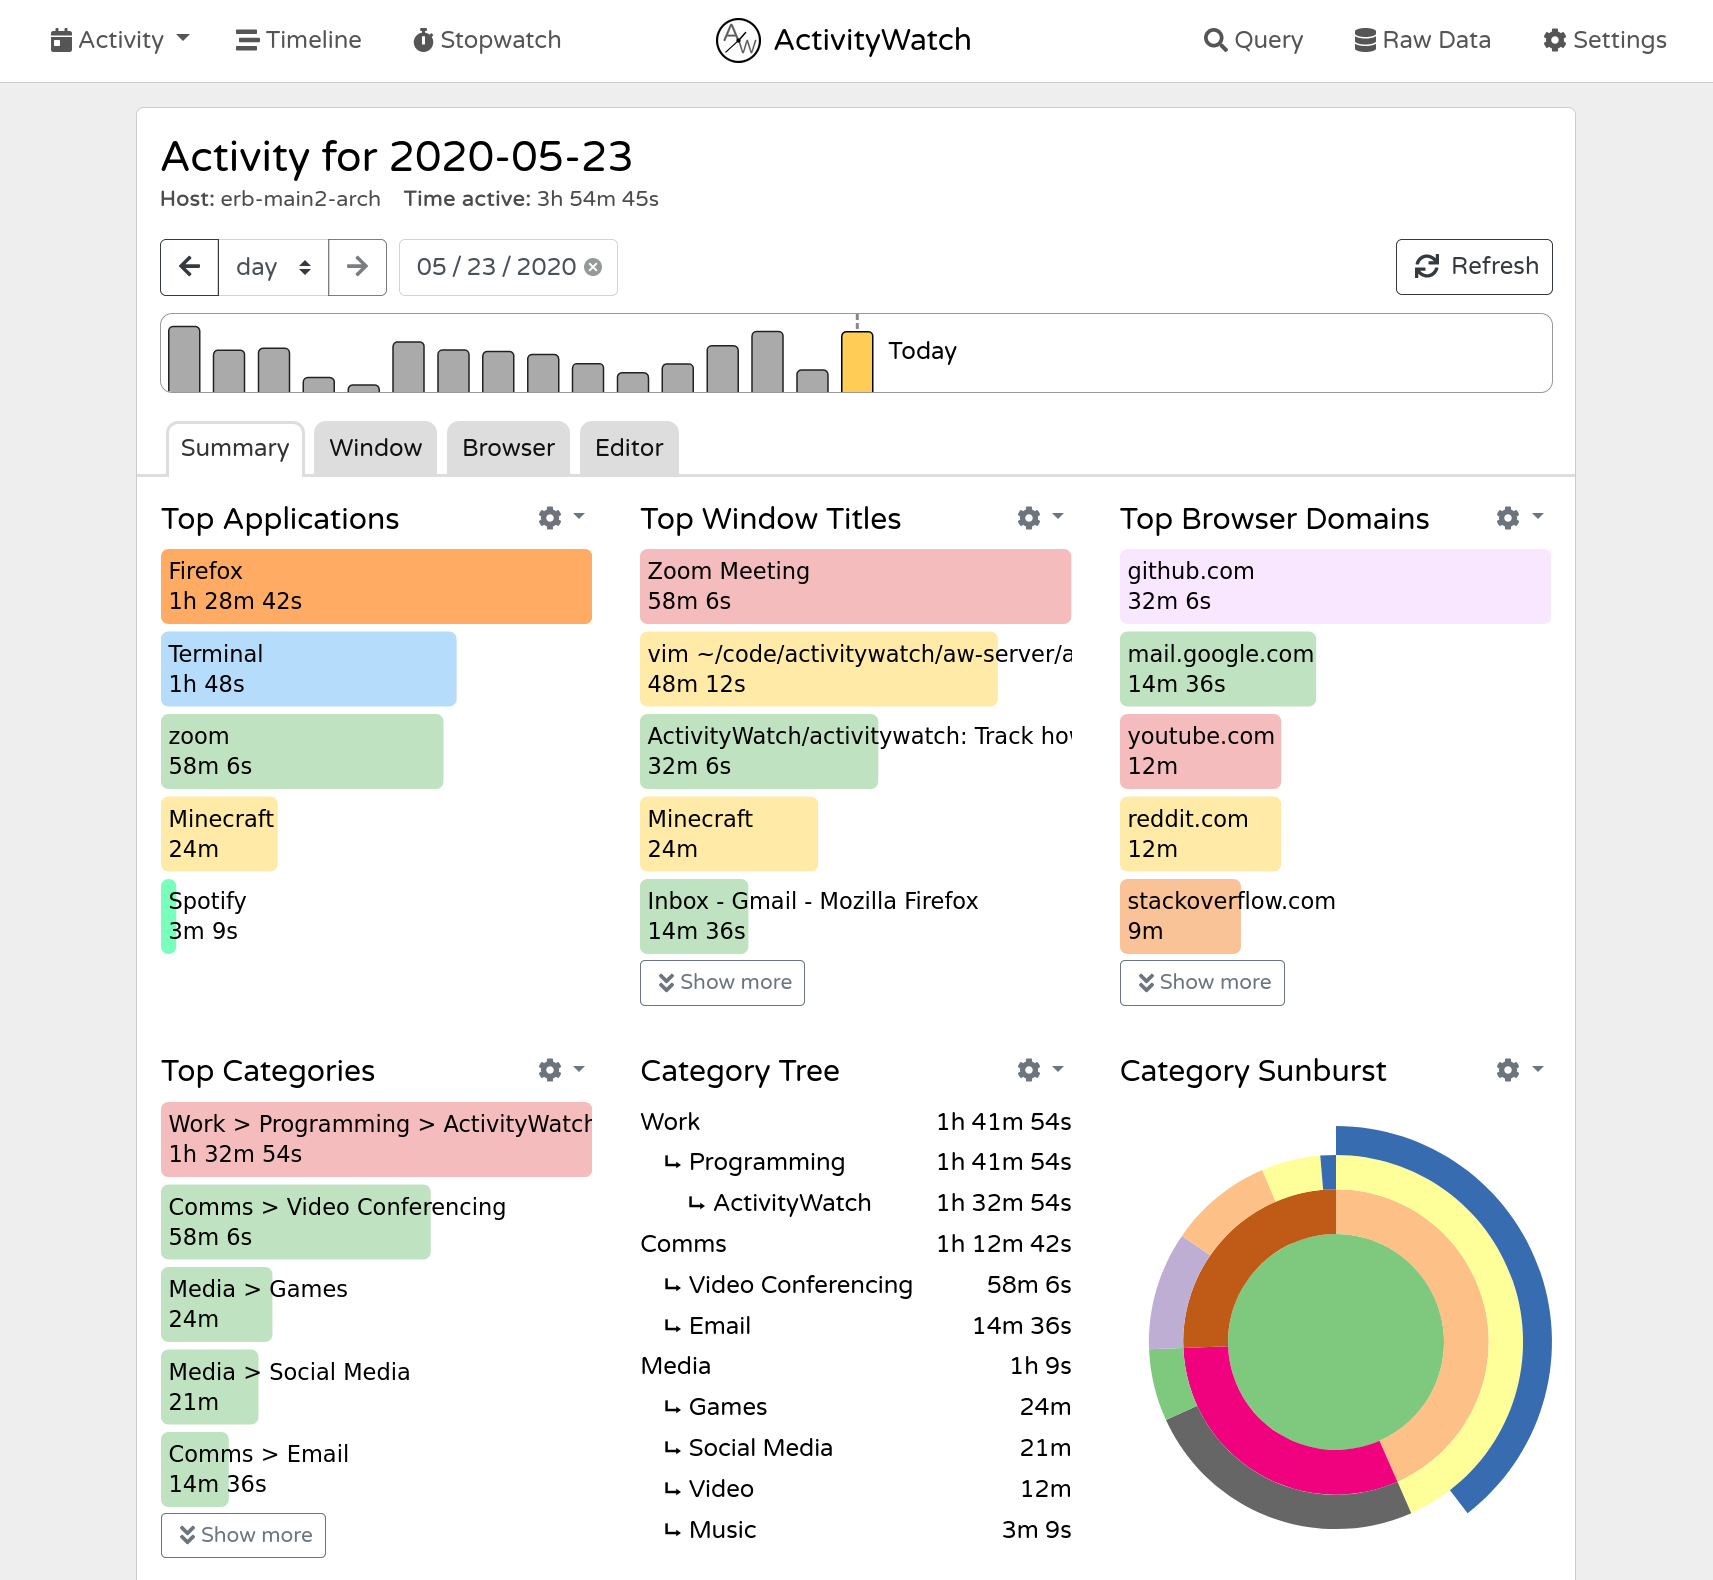
\includegraphics[width=8cm]{img/screenshot-aw-activity.png}
\caption{ActivityWatch activity dashboard. Showing top applications, window titles, browser domains, and categories.}\label{fig:aw}
\end{figure}

%With the advancement of Brain-Computer Interfaces, the relationship between device and brain activity is becoming even more tightly connected.

\subsection{Low-cost functional brain imaging}

Functional brain imaging methods such as fMRI, fNIRS, and EEG, have been used to study the relationship between cognitive or physical activity, and brain activity~\cite{floyd_decoding_2017}\cite{hong_classification_2015}\cite{fucci_replication_2019}. The more accurate methods such as fMRI are costly and inflexible/impractical for many uses.

However, the recent availability of low-cost biosensors such as EEG, HEG, and fNIRS, enables studying brain activity during real-life tasks. As an example it has been shown that it is possible to classify what task a participant is undertaking using fMRI~\cite{floyd_decoding_2017}, which has been replicated using EEG and low-cost biosensors~\cite{fucci_replication_2019}.

But they are not without their limitations --- among them a notably low signal-to-noise ratio~\cite{mcfarland_eeg-based_2017} --- yet visual evoked potentials (VEPs) have been shown to be sufficient for high-speed BCI applications~\cite{spuler_high-speed_2017}.

\add{Paragraph leading into the CNN classifier part}

Convolutional Neural Networks (CNNs) have been successful in classifying time series in general~\cite{zhao_convolutional_2017}, and EEG data in particular~\cite{schirrmeister_deep_2017}. Additionally, Hierarchical Convolutional Neural Networks (HCNNs) have been used for EEG-based emotion recognition~\cite{li_hierarchical_2018}.

% List of functional brain imaging techniques:
%  - fMRI
%  - fNIRS
%  - EEG
%  - HEG

\section{Problem description, research goals and questions}

The aim of this project is to investigate whether EEG and other low-cost biosensors can be used to accurately classify device activity in a broader context than previous studies. This will be useful to future BCI applications where a command might be specific to a particular context.

EEG and other low-cost biosensors have been successful in capturing emotional states. Thus combined tracking of device activity and emotional state can be used to to see study associations between emotional state and device activity. % emotional state device activity causes, or is caused by.

\subsection{Goals}

\begin{itemize}
    \item{TODO}
\end{itemize}

\subsection{Questions}

Can low-cost biosensors like EEG be used to\ldots

\begin{itemize}
    \item Classify which device activity the user is engaging in?
    \item Capture/track emotional states during device use
   %\item Be used to measure flow?
   %\item What about measuring attention/distractibility?
\end{itemize}

\subsection{Challenges}

\begin{itemize}
    \item EEG data collection (limited time for data collection)
    \item Scope creep (hopefully resolved by the time this document is finalized)
    \item TODO
\end{itemize}

\section{Methodology}

We will collect EEG data from subjects during normal device use. Device activity will be recorded and categorized with ActivityWatch. The categorization will be used to train an EEG classifier on device activity.

\section{Scientific contributions}

\begin{itemize}
  \item A EEG classifier for device activity.
  \item Relationships found between device activity and brain activity, as measured by EEG\@.
 %\item The open source automated time-tracker ActivityWatch.
\end{itemize}


\section{Resources}

\begin{itemize}
  \item OpenBCI Cyton biosensing board (8 channel) and Ultracortex headset
  \item HEGduino
  \item Test subjects
 %\item ActivityWatch, an open source automated time tracker (already developed by the author, but never before used in a scientific publication)
\end{itemize}

% References
\bibbysegment{}

% Further reading (uncited)
\nocite{*}
\defbibenvironment{bibnonum}
  {\list{}
     {\setlength{\leftmargin}{\bibhang}%
      \setlength{\itemindent}{-\leftmargin}%
      \setlength{\itemsep}{\bibitemsep}%
      \setlength{\parsep}{\bibparsep}}
  }
  {\endlist}
  {\item}
\printbibliography[notcategory=cited, env=bibnonum, heading=notcited]

\end{document}
